\section{¿Quién está haciendo TDD realmente?} 
\textbf{}\\
\begin{flushleft}
\begin{center}	
\end{center}
\begin{itemize}
\textbf{1.	 “¿Qué tan ágil es TDD?” }
\textbf{}\\
Desafortunadamente, la tasa de adopción de TDD no es tan alta como debería ser realmente.  La siguiente figura resume los resultados del 2010


\textbf{}\\
 La encuesta proporciona información sobre las estrategias de validación que siguen los equipos que dicen ser ágiles. Sospecho que las tasas de adopción informadas para el desarrollador TDD y la aceptación TDD, 53% y 44% respectivamente, son mucho más realistas que las informadas en mi Encuesta sobre el desarrollo impulsado por pruebas (TDD) .

\textbf{}\\

\begin{center}
    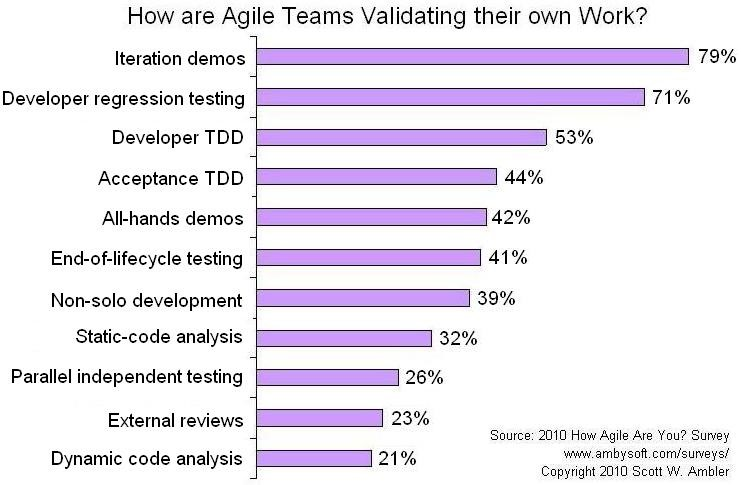
\includegraphics[width=12cm]{./Imagenes/test}
    \end{center}

\end{itemize} 







\end{flushleft}